\documentclass[a4paper]{article}
\usepackage[spanish]{babel}
\usepackage[utf8]{inputenc}
\usepackage{charter}   % tipografia
\usepackage{graphicx}
\usepackage{enumerate}
%\usepackage[]{algorithm2e}
%\usepackage{algorithm}
%\usepackage{algorithmic}[1]
\usepackage{algorithm}
\usepackage{algpseudocode}
%\usepackage{pifont}
\usepackage{listings}
\usepackage{booktabs}
\usepackage{color}
\usepackage{indentfirst}
\usepackage{fancyhdr}
\usepackage{latexsym}
\usepackage{lastpage}
\usepackage{tikz}
\usepackage{subcaption}
\usepackage[colorlinks=true, linkcolor=black]{hyperref}
%\usepackage{makeidx}
%\usepackage{float}
\usepackage{calc}
\usepackage{amsmath, amsthm, amssymb}
\usepackage{amsfonts}
\usepackage{tabularx}
\usepackage{multirow}
\usepackage{makecell}
%\usepackage{sectsty}
%\usepackage{charter}
%\usepackage{wrapfig}
%\usepackage{listings}
%\lstset{language=C}
\definecolor{gray}{gray}{0.5}
\definecolor{light-gray}{gray}{0.95}
\definecolor{orange}{rgb}{1,0.5,0}
%\usepackage{makecell}
%\usepackage{xcolor}
%\usepackage{colortbl}

\usepackage{color} % para snipets de codigo coloreados
\usepackage{fancybox}  % para el sbox de los snipets de codigo

\definecolor{litegrey}{gray}{0.94}

% \newenvironment{sidebar}{%
% 	\begin{Sbox}\begin{minipage}{.85\textwidth}}%
% 	{\end{minipage}\end{Sbox}%
% 		\begin{center}\setlength{\fboxsep}{6pt}%
% 		\shadowbox{\TheSbox}\end{center}}
% \newenvironment{warning}{%
% 	\begin{Sbox}\begin{minipage}{.85\textwidth}\sffamily\lite\small\RaggedRight}%
% 	{\end{minipage}\end{Sbox}%
% 		\begin{center}\setlength{\fboxsep}{6pt}%
% 		\colorbox{litegrey}{\TheSbox}\end{center}}

\newenvironment{codesnippet}{%
	\begin{Sbox}\begin{minipage}{\textwidth}\sffamily\small}%
	{\end{minipage}\end{Sbox}%
		\begin{center}%
		\colorbox{litegrey}{\TheSbox}\end{center}}



\usepackage{fancyhdr}
\pagestyle{fancy}

%\renewcommand{\chaptermark}[1]{\markboth{#1}{}}
\renewcommand{\sectionmark}[1]{\markright{\thesection\ - #1}}

\fancyhf{}

\fancyhead[LO]{Sección \rightmark} % \thesection\ 
\fancyfoot[LO]{\small{Alvarez Mat\'ias, Dorr Francisco, Litwak Brian}}
\fancyfoot[RO]{\thepage}
\renewcommand{\headrulewidth}{0.5pt}
\renewcommand{\footrulewidth}{0.5pt}
\setlength{\hoffset}{-0.8in}
\setlength{\textwidth}{16cm}
%\setlength{\hoffset}{-1.1cm}
%\setlength{\textwidth}{16cm}
\setlength{\headsep}{0.5cm}
\setlength{\textheight}{25cm}
\setlength{\voffset}{-0.7in}
\setlength{\headwidth}{\textwidth}
\setlength{\headheight}{13.1pt}

\renewcommand{\baselinestretch}{1.1}  % line spacing


% \setcounter{secnumdepth}{2}
\usepackage{underscore}
\usepackage{caratula}
\usepackage{url}
\usepackage{float}

\newcommand{\cod}[1]{{\tt #1}}
\newcommand{\negro}[1]{{\bf #1}}
\newcommand{\ital}[1]{{\em #1}}
\newcommand{\may}[1]{{\sc #1}}
\newcommand{\tab}{\hspace*{2em}}

\parskip = 5 pt

\newcounter{row}
\newcounter{col}

\newcommand\setrow[3]{
	\setcounter{col}{1}
	\foreach \n in {#1, #2, #3} {
	\edef\x{\value{col} - 0.5}
	\edef\y{3.5 - \value{row}}
	\node[anchor=center] at (\x, \y) {\n};
	\stepcounter{col}
	}
	\stepcounter{row}
}

\newcommand\setrowaux[7]{
	\setcounter{col}{1}
	\foreach \n in {#1, #2, #3, #4, #5, #6, #7} {
	\edef\x{\value{col} - 0.5}
	\edef\y{7.5 - \value{row}}
	\node[anchor=center] at (\x, \y) {\n};
	\stepcounter{col}
	}
	\stepcounter{row}
}

\newcommand{\real}{\mathbb{R}}

\hypersetup{
 pdfstartview= {FitH \hypercalcbp{\paperheight-\topmargin-1in-\headheight}},
 pdfauthor={Grupo},
 pdfsubject={Dise\~{n}o}
}

\lstdefinestyle{customc}{
  backgroundcolor=\color{light-gray},
  belowcaptionskip=1\baselineskip,
  breaklines=true,
  numbers=left,
  xleftmargin=\parindent,
  language=C,
  showstringspaces=false,
  basicstyle=\footnotesize\ttfamily,
  keywordstyle=\bfseries\color{blue},
  commentstyle=\itshape\color{gray},
  identifierstyle=\color{black},
  stringstyle=\color{orange},
}

\lstdefinestyle{customasm}{
  backgroundcolor=\color{light-gray},
  belowcaptionskip=1\baselineskip,
  numbers=left,
  xleftmargin=\parindent,
  language=[x86masm]Assembler,
  keywordstyle=\bfseries\color{blue},
  basicstyle=\footnotesize\ttfamily,
  commentstyle=\itshape\color{gray},
}

\lstset{escapechar=@}


\begin{document}

\newcolumntype{C}{>{\centering\arraybackslash}X}

\thispagestyle{empty}
\materia{Teoría de las Comunicaciones}
\submateria{Segundo Cuatrimestre de 2015}
\titulo{Trabajo Práctico I}
\subtitulo{\emph{Wiretapping}}
%\grupo{Los heladeros de Gauss}
\integrante{Alvarez, Mat\'ias}{090/12}{matyy.alvarez@gmail.com}
\integrante{Dorr, Francisco}{434/09}{fran.dorr@gmail.com}
\integrante{Litwak, Brian}{241/12}{brian.litwak@gmail.com}
%\fecha{\date{\currentdate}}

\makeatletter
%\renewcommand{\ALG@name}{Algoritmo}

\maketitle
\newpage

\thispagestyle{empty}
\vfill

\thispagestyle{empty}
\vspace{3cm}
\tableofcontents
\newpage

\newenvironment{myindentpar}[1]
{\begin{list}{1}
         {\setlength{\leftmargin}{#1}}
         \item[]
}
{\end{list} }

%\normalsize
\newpage

\section{Objetivo del trabajo}

El objetivo de este trabajo es utilizar técnicas provistas por la teoría de la información para distinguir
diversos aspectos de la red de manera analítica. Para ello, es sugerido el uso de dos herramientas modernas
de manipulación y análisis de paquetes: Wireshark y Scapy.

\subsection{Breve introducción}

En primer lugar implementamos herramientas para simular fuentes de informaci\'on. Una fuente de informaci\'on, desde el punto de vista de la teor\'ia de la informaci\'on de Shannon, es un objeto que emite s\'imbolos $s_i$, en donde cada uno tiene una probabilidad $p_i$ de ser emitido. Entre ellas tendremos:

\begin{itemize}
\item[$\circ$]Una herramienta que simula una fuente que emite paquetes Ethernet, es decir cada s\'imbolo en este caso ser\'a un posible frame generado con dicho protocolo.
\item[$\circ$]Otra herramienta que sumila una fuente que emite paquetes que utilizan el protocolo ARP.
\end{itemize}



\section{Presentaci\'on e hip\'otesis sobre los experimentos}
%\footnote{asd}

Dividiremos la experimentaci\'on del trabajo en tres secciones, en donde cada una consistir\'a en dejar escuchando las herramientas en tres redes distintas. Entre ellas estar\'an las siguientes:

\begin{itemize}
\item[1.] Red hogare\~na: consistir\'a en una peque\~na red en donde tenemos de antemano la noci\'on de cu\'antos equipos pueden estar conectados. En este caso, al ser tres personas las que conviven, sabemos que como m\'aximo se pueden encontrar 7 equipos distintos, entre ellos 3 celulares, 2 tablets, una notebook y un televisor. La duraci\'on de la prueba ser\'a de aproximadamente 6 horas para tener mayor cantidad de informaci\'on, ya que sabemos que la cantidad de equipos que se puede conectar es baja.
\item[2.] Red del laboratorio de computaci\'on: en este caso llevaremos una notebook a la universidad para observar qu\'e cantidad de equipos se conectan en un determinado per\'iodo de tiempo. Sabemos de antemano que entre las 17 y 22hs los laboratorios suelen estar llenos por alumnos de la carrera de computaci\'on, por lo cual cre\'imos que ser\'ia interesante observar lo que sucede en horarios en donde dichos alumnos no acaparan los laboratorios por estar en clase, sino por juntarse para resolver trabajos pr\'acticos, resolver pr\'acticas, etc. Es por esto que la medici\'on se realiz\'o entre las 13 y 14hs.
\item[3.] --
\end{itemize}


Antes de realizar la experimentaci\'on plantearemos algunas hip\'otesis sobre los resultados.

\begin{itemize}
\item[$\circ$]En general creemos que la direcci\'on MAC de broadcast (FF:FF:FF:FF:FF:FF) ser\'a la m\'as pedida, ya que es la direcci\'on en donde los hosts pueden mandar mensajes a todos los dem\'as equipos. %Agregar chamuyo
\item[$\circ$]De la misma forma, en general, creemos que habr\'a una cantidad similar de protocolos en todas las redes ya que son redes p\'ublicas a las que acceden la mayor\'ia de los equipos cotidianos como ser computadoras, celulares y tablets.
\item[$\circ$]En la red hogare\~na creemos que habr\'a poca cantidad de env\'io de paquetes ARP \textit{who is} dado que la cantidad de dispositivos es muy acotada.
\item[$\circ$]En la red del laboratorio creemos que esto \'ultimo ser\'a al rev\'es, es decir, habr\'a mucho env\'io de paquetes ARP \textit{who is} de distintas MAC, pues la mayor cantidad de conexiones suele provenir de celulares y \'estos tienden a bloquearse y desbloquearse cada poco tiempo (y cada vez que se realiza esa acci\'on, la gran mayor\'ia de los celulares apaga el wifi de a momentos para ahorrar bater\'ia). Por lo cual cada reconexi\'on implica una nueva tanda de mensajes ARP y es por esto que creemos que la cantidad final ser\'a muy elevada.
\item[$\circ$] --
\end{itemize}

Las hip\'otesis generales ser\'an corroboradas en el final del informe y las que dependen de cada red, al final de cada experimentaci\'on.


\section{Experimentaci\'on}

\subsection{Red hogare\~na}

Comenzaremos la experimentaci\'on recolectando datos sobre la cantidad y diversidad de protocolos.

\begin{figure}[h!]
\centering
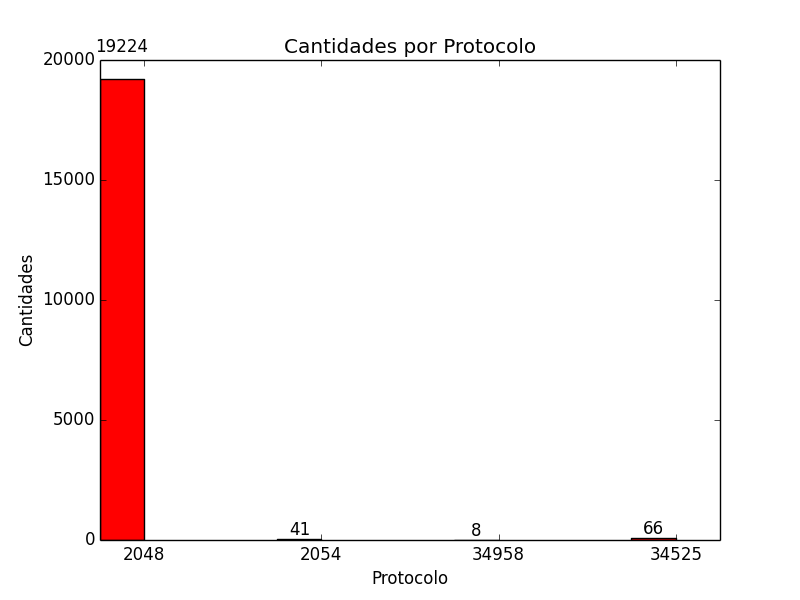
\includegraphics[width=0.7\linewidth]{imagenes/exp1/1cantidadProtocolo}
\caption{Distintos tipos de protocolos (EtherType) encontrados en la red, organizados por cantidad}
\label{exp1grafico1}
\end{figure}

En primer lugar vemos que se cuenta con una peque\~na cantidad de protocolos y cuando buscamos en la lista de EtherTypes de IEEE\footnote{http://www.iana.org/assignments/ieee-802-numbers/ieee-802-numbers.xhtml} encontramos que el c\'odigo 2048 pertenece a mensajes de tipo \textit{IPv4}, el 2054 a mensajes \textit{ARP}, el 34958 a lo que se denomina como \textit{Portbased network access protocol} y el 34983 a \textit{Service VLAN tag identifier}.\newline

El gr\'afico resulta bastante intuitivo ya que la mayor\'ia de los mensajes que emite un dispositivo cotidiano como ser un celular o una computadora suelen ser paquetes IP que viajan por internet para realizar pedidos, por lo cual son de tipo IPv4 (que es el modo utilizado en la actualidad) y esto explica la gran cantidad de estos paquetes. Por otro lado, la proporci\'on de ARP resulta muy baja debido a la cantidad de dispositivos que existen en la red. Los otros protocolos, creemos que son necesarios por el router de la casa por la configuraci\'on del proveedor de servicios.


\newpage

Veamos a continuaci\'on el mismo gr\'afico detallando las probabilidades de cada s\'imbolo (protocolo).

\begin{figure}[h!]
\centering
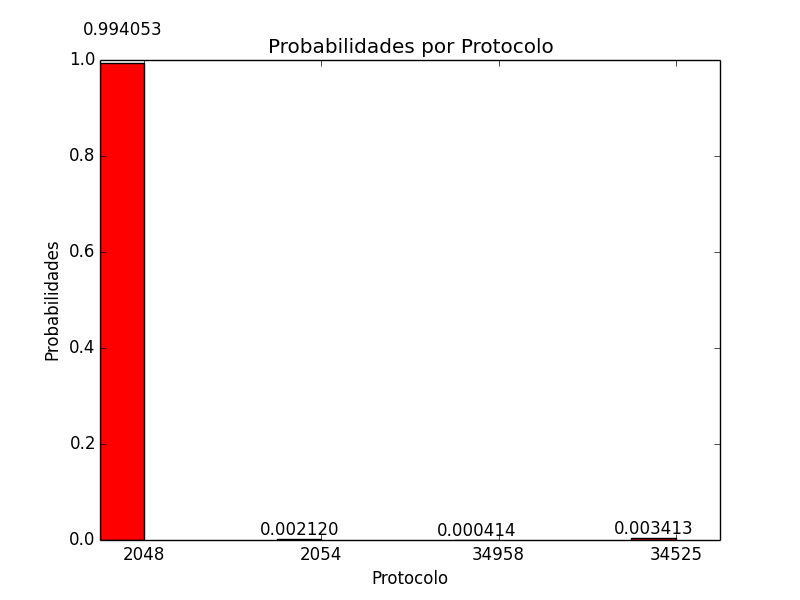
\includegraphics[width=0.7\linewidth]{imagenes/exp1/2probabilidadProtocolo}
\caption{Probabilidad por cada tipo de protocolo detectado}
\label{exp1grafico1}
\end{figure}

La proporci\'on de paquetes ARP por sobre el resto de los paquetes termina siendo del 0.0021\% , lo que en principio podr\'ia indicarnos que tiene una fuerte relaci\'on con la baja cantidad de dispositivos (es decir, lo que ya sabemos desde la teor\'ia).\newline

Veamos a continuaci\'on el gr\'afico de la entrop\'ia a medida que se transmiten paquetes.


\begin{figure}[h!]
\centering
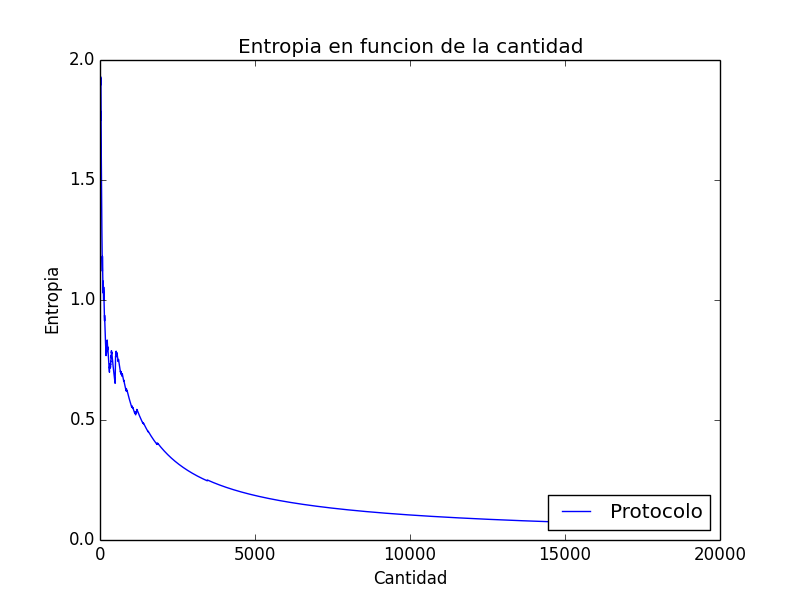
\includegraphics[width=0.7\linewidth]{imagenes/exp1/3entropiaProtocolo}
\caption{Entrop\'ia a medida que aumenta la cantidad de s\'imbolos emitidos por la fuente}
\label{exp1grafico1}
\end{figure}


Podemos ver que la entrop\'ia se relaciona con la cantidad y con la probabilidad pues sabemos por la teor\'ia de la informaci\'on de Shannon que cuando una fuente emite con mucha probabilidad un s\'imbolo, se vuelve poco informativa, dado que lo que \'esta puede emitir se vuelve muy predecible. Lo mismo aplica en este caso para los paquetes IPv4.\newline

Por otro lado vemos que la entrop\'ia comienza siendo muy alta, lo que puede indicar que en un principio habr\'ia una proporci\'on similar de probabilidades entre los protocolos, pero a la larga el protocolo IPv4 domina la red y la fuente se vuelve altamente predecible, por lo cual la entrop\'ia decrece fuertemente.\newline


Veamos a continuaci\'on lo que sucedi\'o con los env\'ios de paquetes IP desde y hacia los hosts.




\begin{figure}[H]

\begin{subfigure}{0.6\textwidth}
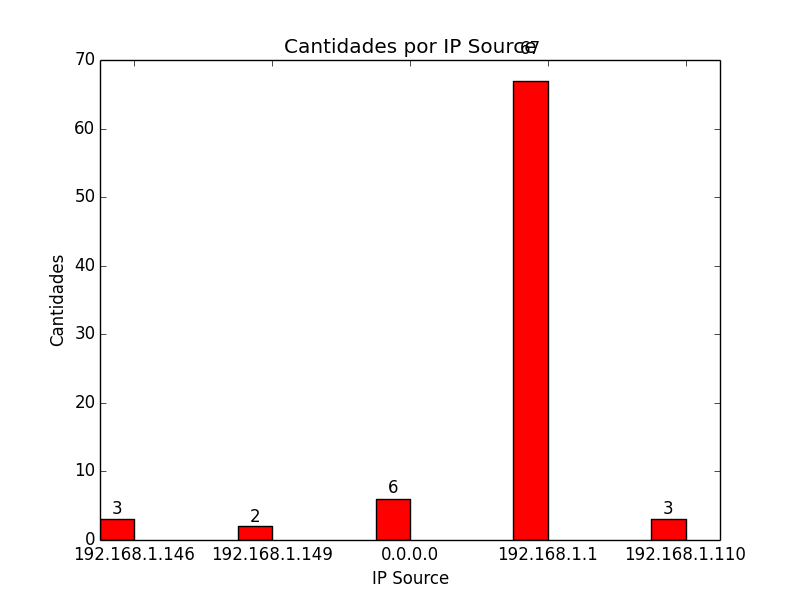
\includegraphics[width=0.9\linewidth, height=6cm]{imagenes/exp1/4cantidadIPSource} 
\caption{}
\end{subfigure}
\begin{subfigure}{0.6\textwidth}
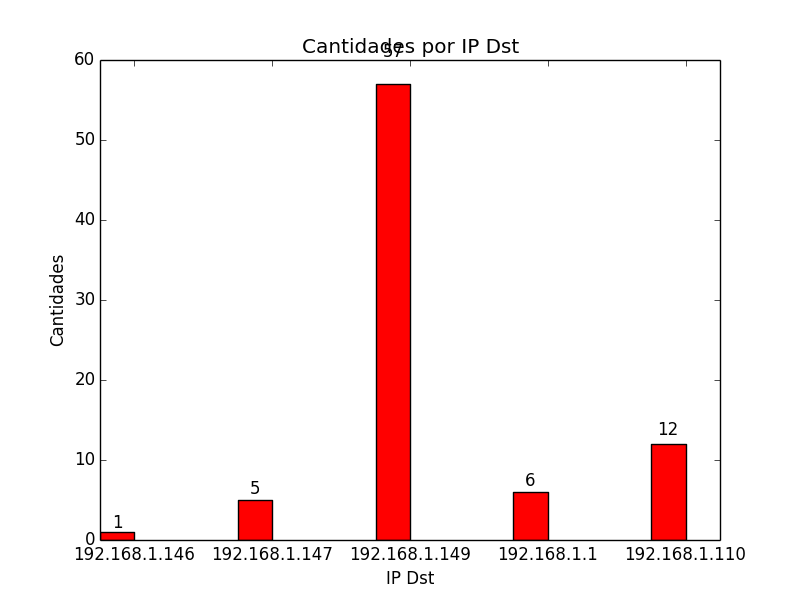
\includegraphics[width=0.9\linewidth, height=6cm]{imagenes/exp1/5cantidadIPDst}
\caption{}
\end{subfigure}

\caption{Direcciones IP asignadas en la red}
\label{fig:1}
\end{figure}

En esta figura podemos ver que la mayor cantidad del tr\'afico se lo llevan las direcciones 192.168.1.1 y 192.168.1.149, en donde claramente se ve que interact\'uan fuertemente entre ellas. Creemos que esto representa el tr\'afico entre la notebook y el router, para acceder a contenidos de internet. Los dem\'as equipos presentan un rol m\'as pasivo y tiene correspondencia con el hecho de ser celulares o tablets en un ambiente hogare\~no.\newline

Visto de otro modo, las probabilidades de estos mensajes resultaron las siguientes.

\begin{figure}[H]

\begin{subfigure}{0.6\textwidth}
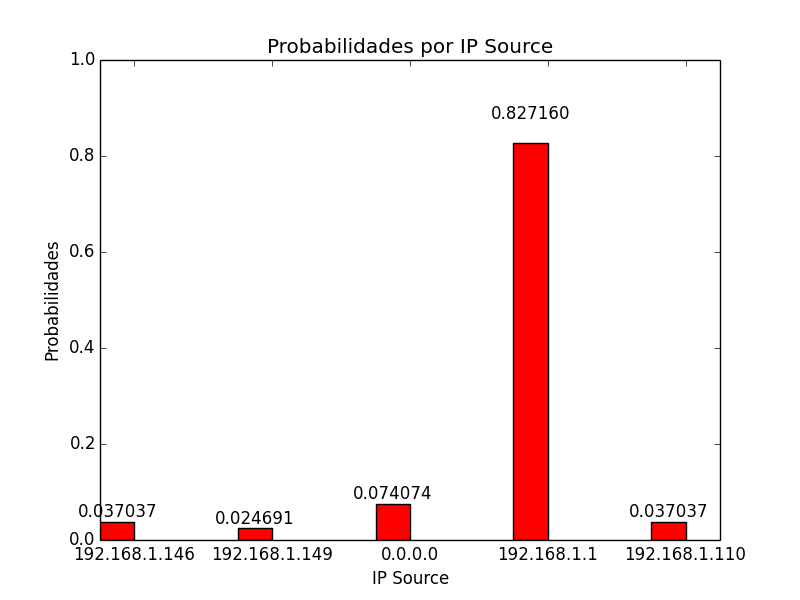
\includegraphics[width=0.9\linewidth, height=6cm]{imagenes/exp1/6probabilidadIPSource} 
\caption{}
\end{subfigure}
\begin{subfigure}{0.6\textwidth}
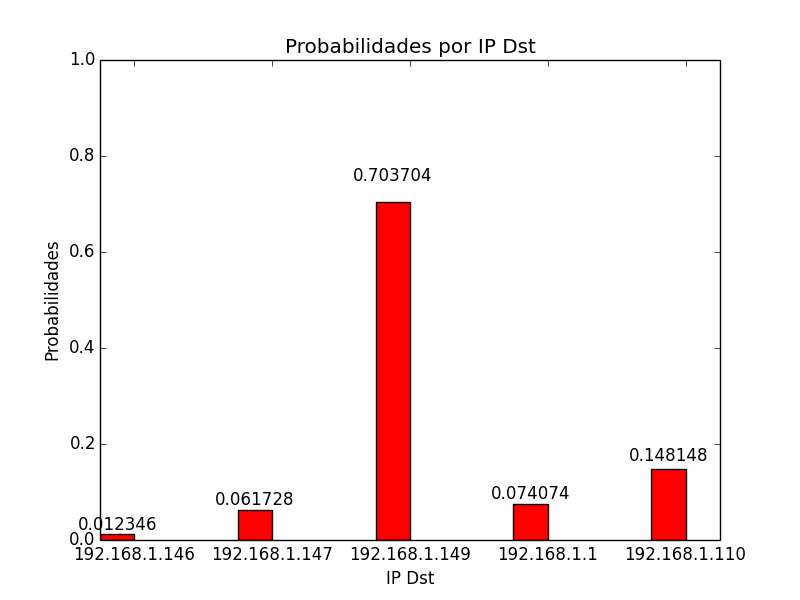
\includegraphics[width=0.9\linewidth, height=6cm]{imagenes/exp1/7probabilidadIPDst}
\caption{}
\end{subfigure}

\caption{Probabilidades correspondientes a los paquetes IP origen y destino}
\label{fig:1}
\end{figure}

Comparando los gr\'aficos de origen y destino podemos ver que los dem\'as equipos efectivamente tienen un rol pasivo ya que se les env\'ia bastantes m\'as paquetes de los que ellos mandan.\newline

Veamos la entrop\'ia de la red.

\begin{figure}[h!]
\centering
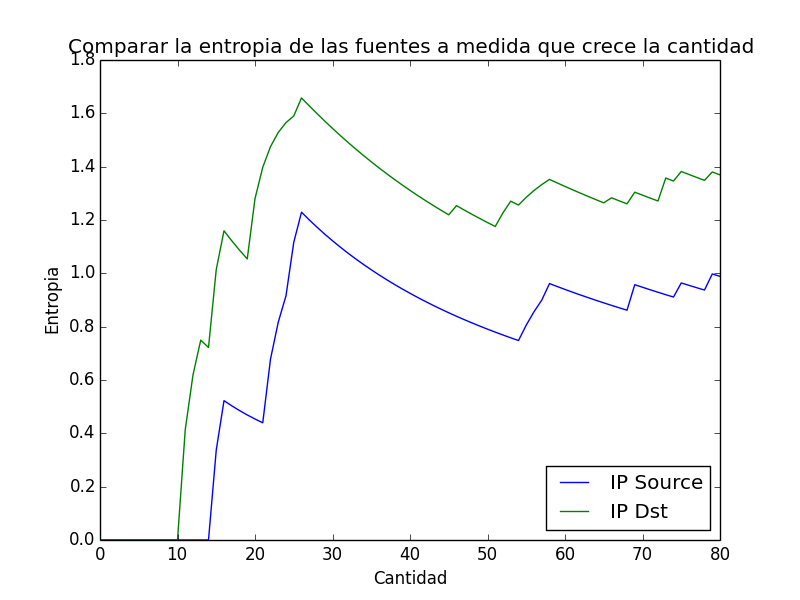
\includegraphics[width=0.7\linewidth]{imagenes/exp1/8entropiaIPDstyIPSource}
\caption{Entrop\'ia a medida que aumenta la cantidad de s\'imbolos emitidos por la fuente}
\label{exp1grafico1}
\end{figure}

El gr\'afico presenta un comportamiento particular que no observamos anteriormente. En principio creemos que comienza con un valor de 0 y se estanca por un tiempo ya que ning\'un dispositivo tuvo actividad en la red en ese intervalo (lo cual es entendible sabiendo que hay pocos dispositivos). En cuanto se detecta actividad sube fuertemente la entrop\'ia y desde ah\'i comienza a bajar y subir con un patr\'on similar. La explicaci\'on que encontramos a esto es que en esos picos es cuando se pelean las direcciones 192.168.1.1 y 192.168.1.149 en mandarse mensajes entre ellas. Cuando se env\'ian la misma cantidad de mensajes la entrop\'ia sube (ya que crece la incertidumbre), luego una de ellas emite m\'as que la otra y la entrop\'ia baja, luego se vuelven a nivelar y as\'i sucesivamente.\newline

El mapa de la red qued\'o representado de la siguiente forma.

\begin{figure}[h!]
\centering
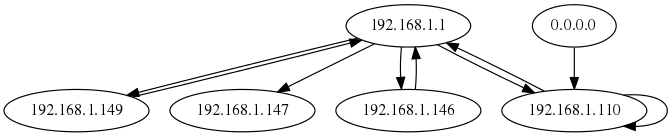
\includegraphics[width=0.7\linewidth]{imagenes/exp1/IPnodos}
\caption{Grafo de conexiones (por env\'io de mensajes) de la red hogare\~na}
\label{exp1grafico1}
\end{figure}

\newpage

Por \'ultimo veamos c\'omo qued\'o el env\'io distribu\'ido por direcciones MAC.

\begin{figure}[H]

\begin{subfigure}{0.6\textwidth}
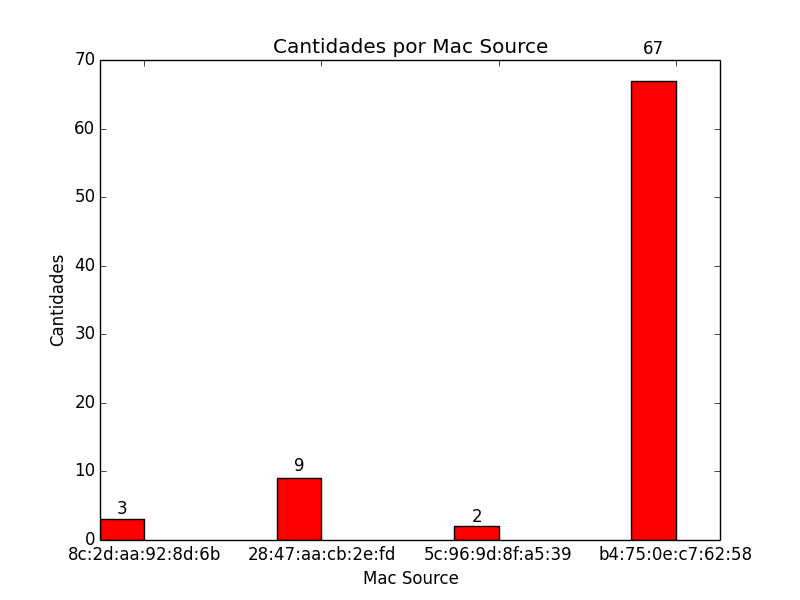
\includegraphics[width=0.9\linewidth, height=6cm]{imagenes/exp1/9cantidadMacSource} 
\caption{}
\end{subfigure}
\begin{subfigure}{0.6\textwidth}
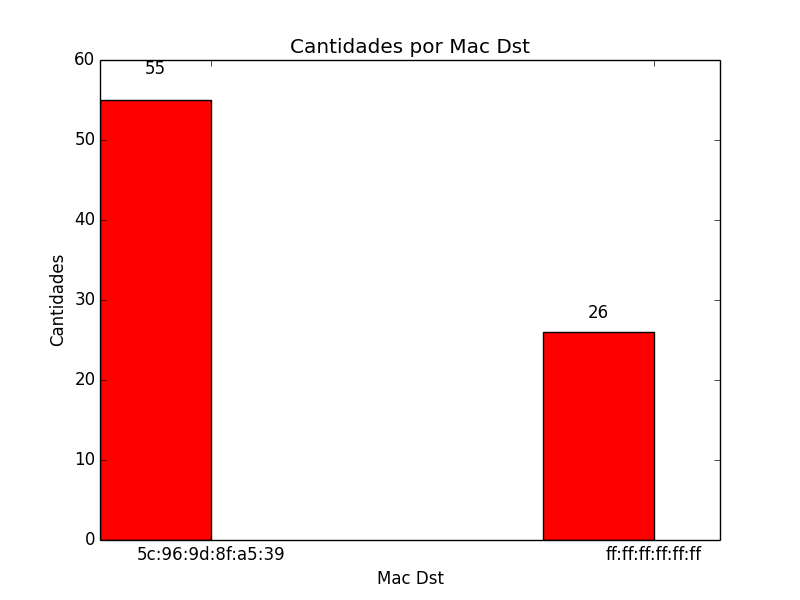
\includegraphics[width=0.9\linewidth, height=6cm]{imagenes/exp1/10cantidadMacDst}
\caption{}
\end{subfigure}

\caption{Direcciones MAC asignadas en la red}
\label{fig:1}
\end{figure}

En este gr\'afico aparecen menos hosts que en el caso de paquetes IP. Esto, creemos, es porque el router reasigna direcciones IP distintas a un mismo equipo cada vez que se conecta, por lo cual la direcci\'on MAC que env\'ia es siempre la misma.

\begin{figure}[H]
\begin{subfigure}{0.6\textwidth}
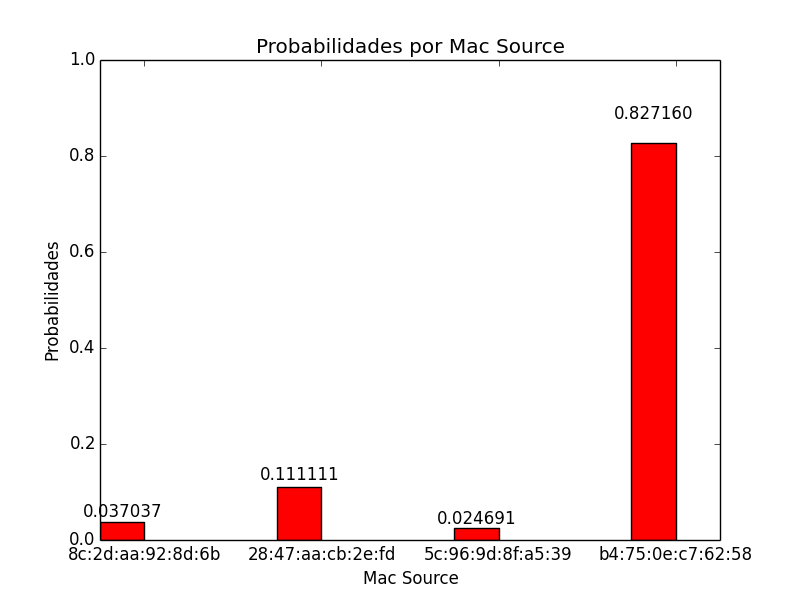
\includegraphics[width=0.9\linewidth, height=6cm]{imagenes/exp1/11probabilidadMacSource} 
\caption{}
\end{subfigure}
\begin{subfigure}{0.6\textwidth}
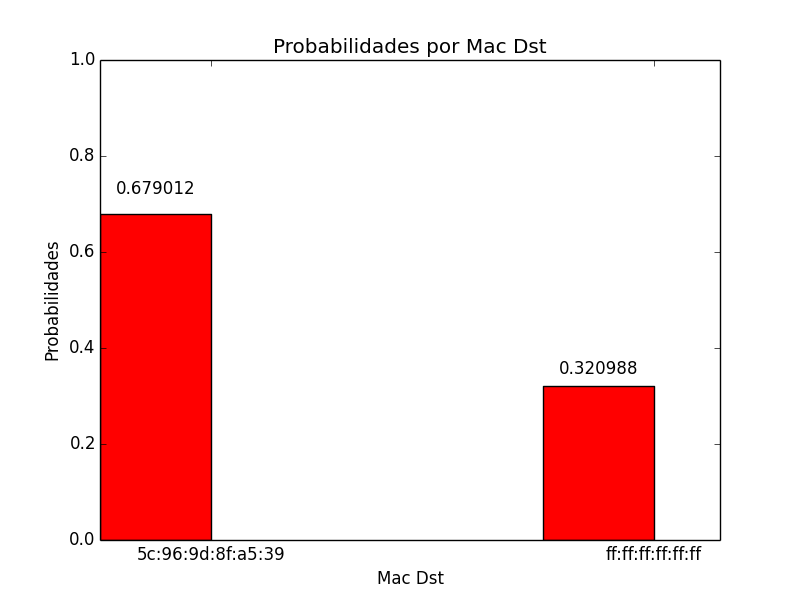
\includegraphics[width=0.9\linewidth, height=6cm]{imagenes/exp1/12probabilidadMacDst}
\caption{}
\end{subfigure}
\caption{Probabilidad por cada direcci\'on MAC de la red de aparecer en un mensaje}
\label{fig:1}
\end{figure}

\newpage

Por \'ultimo veamos la entrop\'ia de la fuente.

\begin{figure}[h!]
\centering
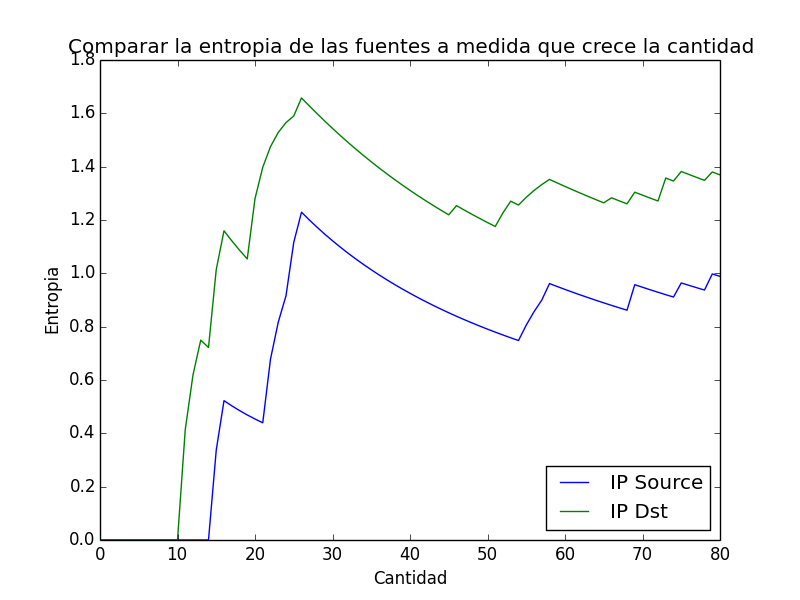
\includegraphics[width=0.7\linewidth]{imagenes/exp1/8entropiaIPDstyIPSource}
\caption{Entrop\'ia a medida que aumenta la cantidad de s\'imbolos emitidos por la fuente}
\label{exp1grafico1}
\end{figure}

Este gr\'afico presenta una tendencia similar a la de la entrop\'ia por direcci\'on IP, con una curvatura en el pico de la MAC destino que antes se presentaba entre los 25 y 30 paquetes. Este fen\'omeno creemos que puede deberse a dos dispositivos que en ese momento cambiaron a la misma IP que present\'o el pico (porque alguno se desconect\'o o reconect\'o, por ejemplo) y sin embargo en las direcciones MAC fueron distintas. Por eso la curva de la entrop\'ia por MAC no tuvo un pico tan brusco.\newline
% REVISAR ESTO, MEPA QUE ES CHAMUYO

Para concluir con esta primera experimentaci\'on, podemos rescatar que en una red peque\~na de hogar queda corroborado que suele haber poca actividad y la mayor cantidad de paquetes son los IPv4.


\newpage

\subsection{Red del laboratorio de computaci\'on}

Veamos en primer lugar datos sobre la cantidad y diversidad de protocolos de esta red. Queremos remarcar en primer lugar que, al haber muchos equipos, a modo de mostrar gr\'aficos m\'as legibles, dejamos en vista s\'olo las direcciones IP y MAC que cumplieron haber mandado al menos 100 mensajes (de lo contrario terminaban siendo al rededor de 80 equipos distintos, muchos con un tr\'afico insignificante, y los resultados se volv\'ian ilegibles). Adem\'as, en los gr\'aficos de probabilidad mostramos los equipos con al menos 0.02\% de los mensajes de la red.\newline

Comenzando con la distinci\'on por protocolos, sabemos que esta es una red que interact\'ua con muchos dispositivos distintos y por lo tanto podr\'ia presentar m\'as protocolos de lo normal. Veamos qu\'e es lo que arrojaron los resultados.

\begin{figure}[h!]
\centering
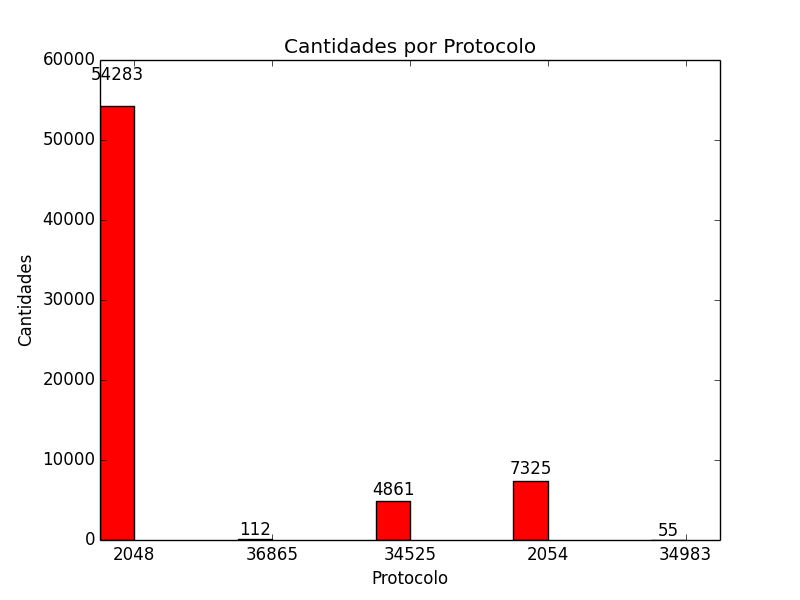
\includegraphics[width=0.7\linewidth]{imagenes/exp2/1cantidadProtocolo}
\caption{Distintos tipos de protocolos (EtherType) encontrados en la red, organizados por cantidad}
\label{exp1grafico1}
\end{figure}

Lo que muestra la figura es que, al igual que en la red hogare\~na, aparecen muy pocos protocolos. Esta vez, en cambio, la proporci\'on de mensajes IPv4 (EtherType 2048) no llega a ser tan desmedida con mensajes de protocolo ARP (EtherType 2054) y de IPv6 (EtherType 34525). Por lo cual la proporci\'on del protocolo ARP sobre la red es del 0,0729\% (comparado con el 0,0021\% del experimento anterior).\newline

Esto le da credibilidad a la hip\'otesis que planteamos de que la gente en este ambiente suele conectar y desconectar mucho los aparatos de la red, y suele usarla durante peque\~nos lapsos.\newline

\newpage

Veamos la misma figura mostrando los respectivos porcentajes.

\begin{figure}[h!]
\centering
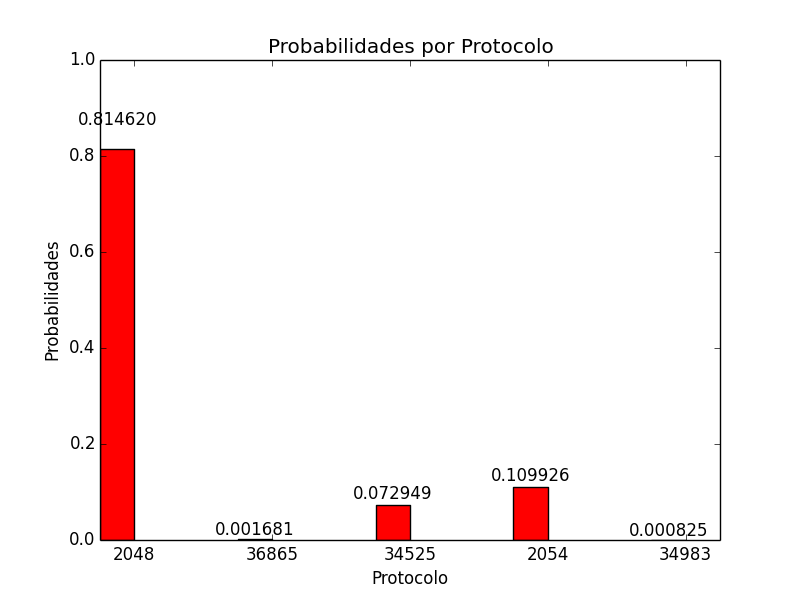
\includegraphics[width=0.7\linewidth]{imagenes/exp2/2probabilidadProtocolo}
\caption{Probabilidad por cada tipo de protocolo detectado}
\label{exp1grafico1}
\end{figure}

Esta baja respecto del porcentaje de mensajes de protocolo IP nos hace notar la idea hablada en clase de que a medida que aumentan las redes (es decir, aumenta la cantida de equipos de una red), comienza a haber m\'as tr\'afico de paquetes para sincronizar y organizar y menos de paquetes con informaci\'on de verdad. Lo cual nos hace comprender por qu\'e es que conviene limitar la cantidad de computadoras en una misma red.

Veamos qu\'e sucedi\'o con la entrop\'ia.

\begin{figure}[h!]
\centering
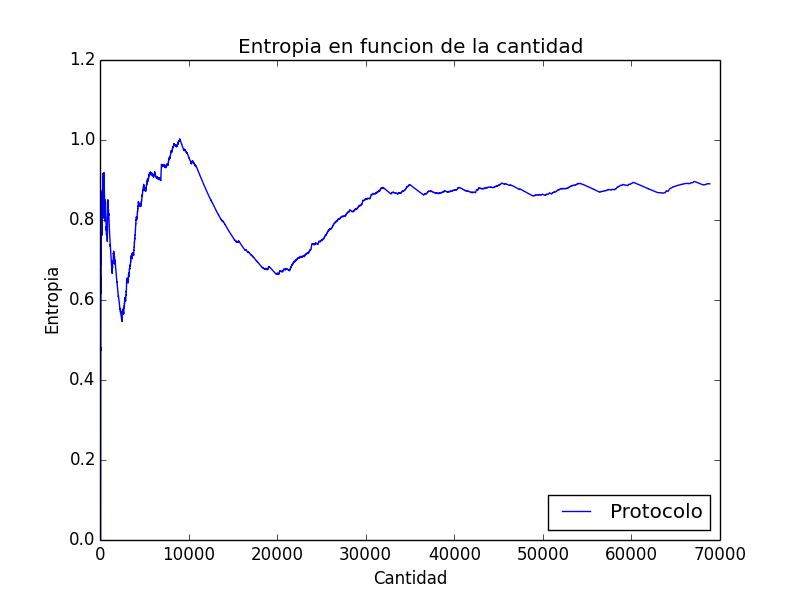
\includegraphics[width=0.7\linewidth]{imagenes/exp2/3entropiaProtocolo}
\caption{Entrop\'ia a medida que aumenta la cantidad de s\'imbolos emitidos por la fuente}
\label{exp1grafico1}
\end{figure}

Si bien se puede ver que oscila, la tendencia parece ser de estancarse en un mismo valor. Es decir, no parece haber mayores picos ni competencia de popularidad (por as\'i decirlo) por parte de varios equipos. S\'i notamos que la entrop\'ia tiene un valor bajo y esto podr\'ia indicar que hay un equipo (o muy pocos) que siempre env\'ian mensajes.\newline


Veamos esto con los gr\'aficos de los env\'ios de paquetes IP desde y hacia los hosts.

\begin{figure}[h!]
\centering
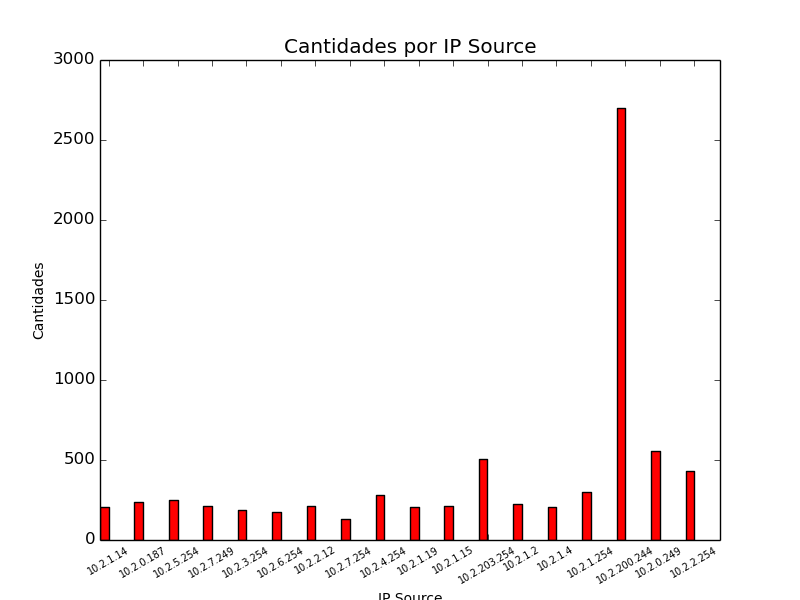
\includegraphics[width=0.7\linewidth]{imagenes/exp2/4v2CantidadesIPSource100}
\caption{Mensajes con IP origen en la red}
\label{exp1grafico1}
\end{figure}

\begin{figure}[h!]
\centering
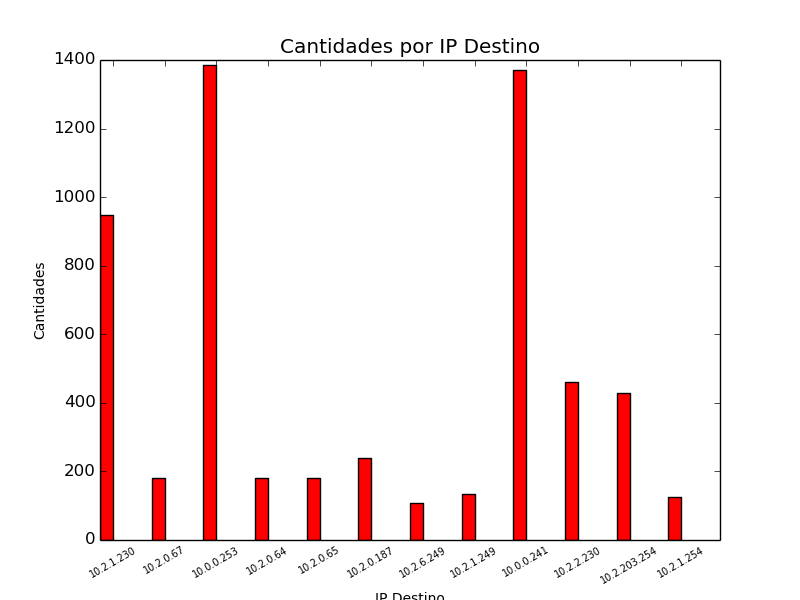
\includegraphics[width=0.7\linewidth]{imagenes/exp2/5v2CantidadesIPDestino100}
\caption{Mensajes con IP destino en la red}
\label{exp1grafico1}
\end{figure}


En esta figura podemos ver que la mayor cantidad del tr\'afico de env\'io se lo lleva la direcci\'on 10.2.1.254, con una fuerte desigualdad respecto al resto de dispositivos. Esto podr\'ia representar a un usuario que utiliz\'o una notebook y que estuvo navegando en internet la mayor parte del tiempo en que dur\'o el experimento. Por otro lado el tr\'afico de recepci\'on estuvo apenas un poco m\'as compartido, por 3 equipos que se distinguieron (10.2.1.230, 10.0.0.253 y 10.0.0.241, entre los cuales no aparece el host anteriormente mencionado).

\newpage
Visto de otro modo, las probabilidades de estos mensajes resultaron las siguientes.

\begin{figure}[H]

\begin{subfigure}{0.6\textwidth}
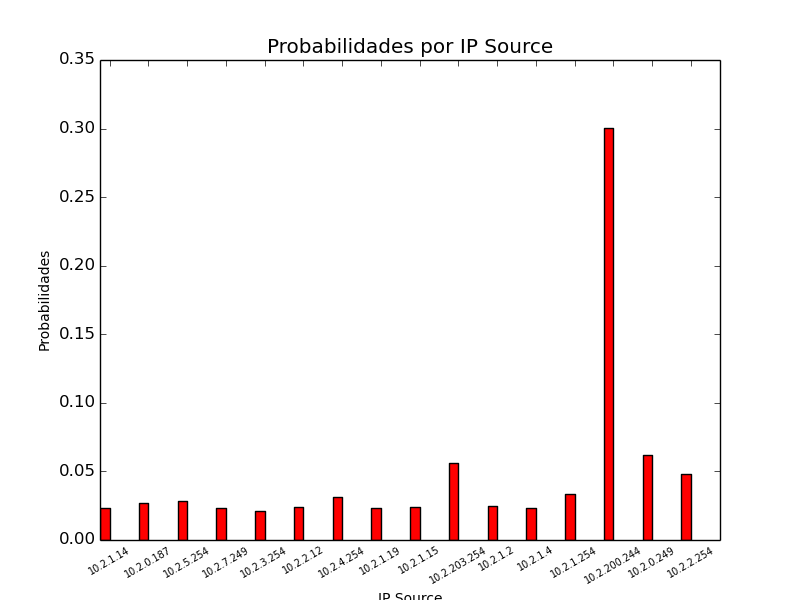
\includegraphics[width=0.9\linewidth, height=6cm]{imagenes/exp2/6v2ProbabilidadesIPSource} 
\caption{}
\end{subfigure}
\begin{subfigure}{0.6\textwidth}
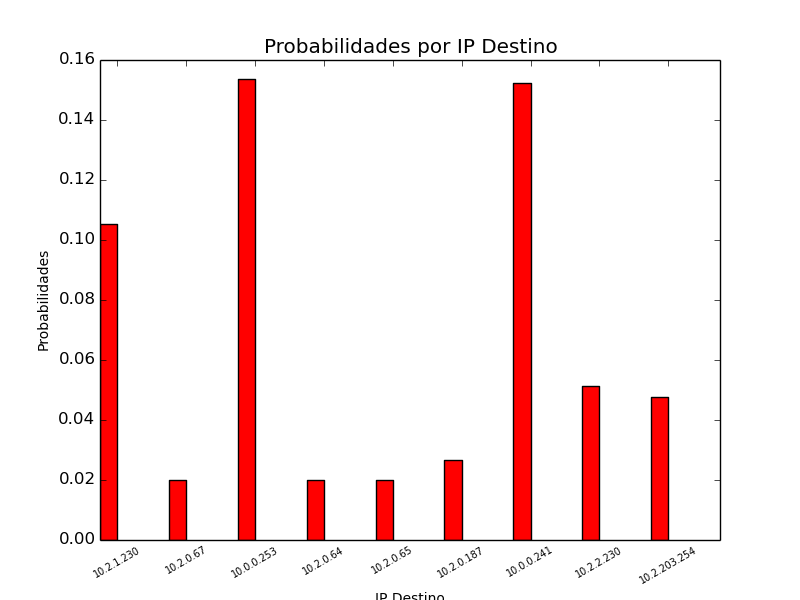
\includegraphics[width=0.9\linewidth, height=6cm]{imagenes/exp2/7v2ProbabilidadesIPDestino}
\caption{}
\end{subfigure}

\caption{Probabilidades correspondientes a los paquetes IP origen y destino}
\label{fig:1}
\end{figure}

Comparando los porcentajes se ve que en general el uso que le da cada host a la red suele ser equitativo, exceptuando algunos outliers que acaparan la red en su totalidad. Esta desigualdad tan grande con el o los outliers puede ocasionar que la fuente igualmente pierda incertidumbre y por lo tanto la entrop\'ia sea baja. Veamos justamente c\'omo se comport\'o la entrop\'ia en el siguiente gr\'afico.

\begin{figure}[h!]
\centering
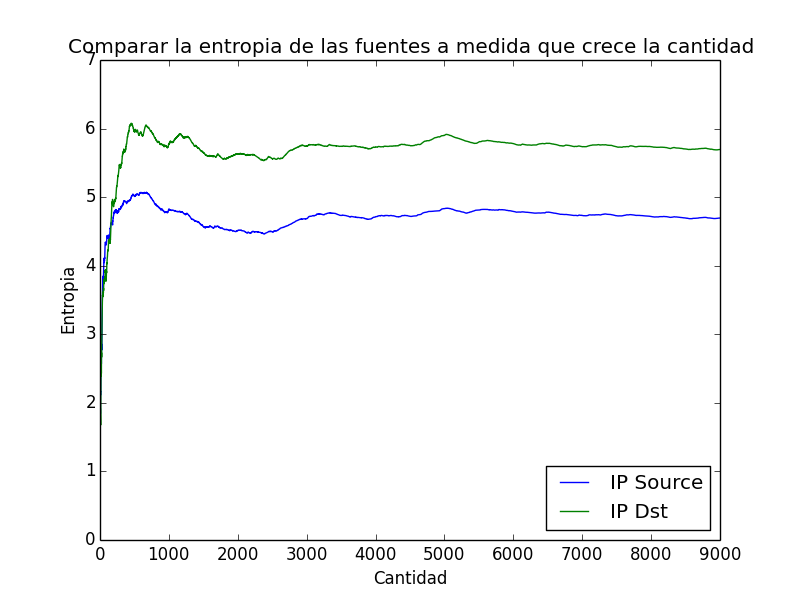
\includegraphics[width=0.7\linewidth]{imagenes/exp2/8entropiaIPDstyIPSource}
\caption{Entrop\'ia a medida que aumenta la cantidad de s\'imbolos emitidos por la fuente}
\label{exp1grafico1}
\end{figure}

Contradiciendo lo que pens\'abamos en un principio, la entrop\'ia result\'o tener un valor elevado. Esto creemos que se debe a que la suma de todos los hosts termina consiguiendo un porcentaje bastante superior al del outlier (donde este \'ultimo tuvo aproximadamente 0.31\% en el caso de IP origen). Por otro lado la entrop\'ia sigui\'o estable a trav\'es de todo el experimento por lo cual no hubo momentos en los cuales un equipo acapar\'o totalmente la red. Eso habla bien del nivel de fairness de uso de la red.\newpage

Por \'ultimo veamos qu\'e sucedi\'o desde el punto de vista de las direcciones MAC.

\begin{figure}[h!]
\centering
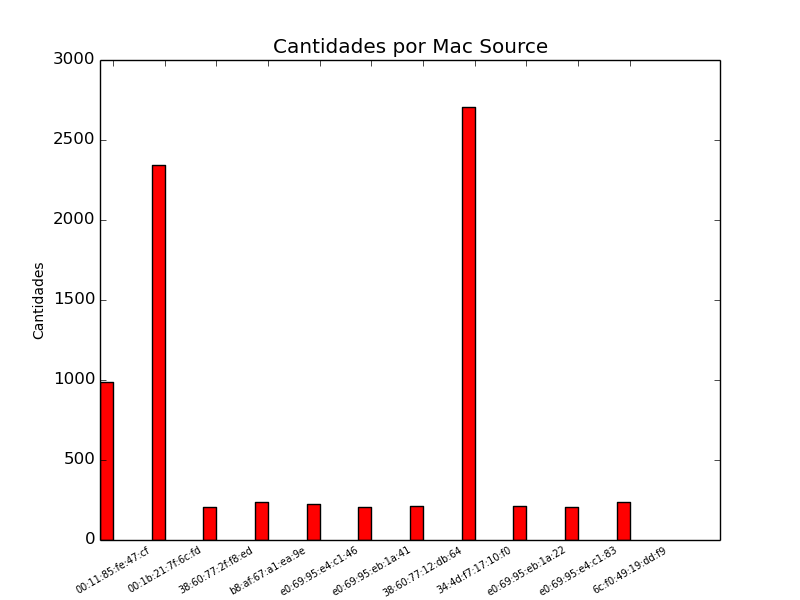
\includegraphics[width=0.7\linewidth]{imagenes/exp2/9v2CantidadesMacSource100}
\caption{Mensajes de direcciones MAC origen en la red}
\label{exp1grafico1}
\end{figure}

En este caso aparecieron menos cantidad de dispositivos a lo largo de toda la hora en la que se utiliz\'o la herramienta. Adem\'as y por lo que se puede ver en el gr\'afico, aparecieron m\'as de una direcci\'on dominante (el outlier del que habl\'abamos antes) y esto nos muestra que dos direcciones MAC muy activas tomaron la misma direcci\'on IP al desconectarse y conectarse. Es por esta suma que se origin\'o el gran outlier antes mencionado. Por otro lado, el tercer dispositivo con mayor cantidad en esta figura muestra un env\'io de 1000 paquetes, cuando anteriormente vimos que ninguna direcci\'on IP (que no fuera la distinguida) enviaba m\'as de 200 paquetes. Esto explica que ese host se conect\'o y desconect\'o al menos unas 5 veces en medio de todo el intervalo de tiempo.\newline

Por \'ultimo veamos la entrop\'ia de la fuente.

\begin{figure}[h!]
\centering
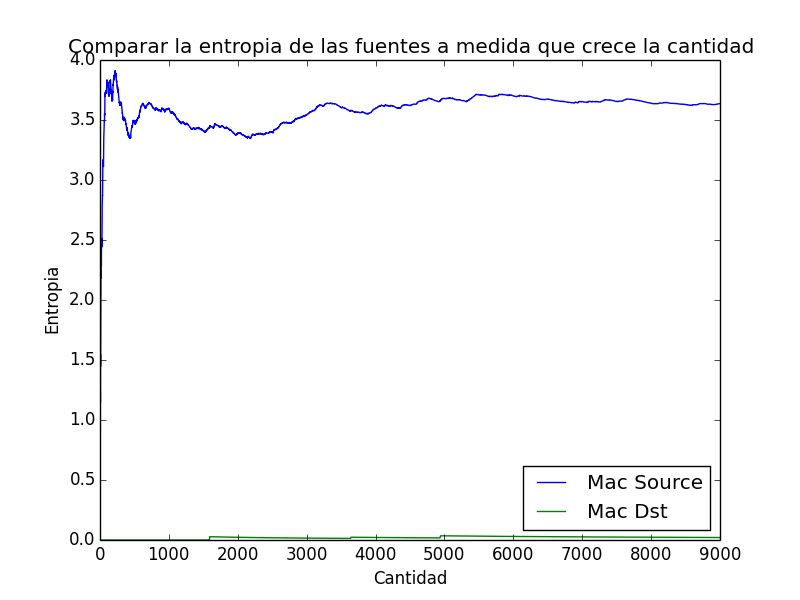
\includegraphics[width=0.7\linewidth]{imagenes/exp2/10entropiaMacDstyMacSource}
\caption{Entrop\'ia a medida que aumenta la cantidad de s\'imbolos emitidos por la fuente}
\label{exp1grafico1}
\end{figure}

Este gr\'afico muestra la misma tendencia que hubo con las direcciones IP: un valor alto dado que hay incertidumbre por parte de la fuente, y un valor que se estanca en el tiempo, indicando que no hay un momento espec\'ifico en que un usuario pasa de ser inactivo a dominar la red.\newline
% FALTA GRAFO

Para concluir esta segunda parte, podemos rescatar varias ideas:

\begin{itemize}
\item[$\circ$]Durante el mediod\'ia, los laboratorios tienen bastante actividad, aunque no es la actividad que se presenta por la tarde-noche (despu\'es de las 17hs). Notamos que a lo largo de la hora en la que ejecutamos la herramienta, se conectaron m\'as de 80 equipos distintos y eso equivale a dos laboratorios completamente ocupados. En comparaci\'on, por la noche suelen llenarse los 6 laboratorios.
\item[$\circ$]Suele haber mucho m\'as tr\'afico de paquetes ARP y de otros protocolos que en una red hogare\~na habitual, por lo cual tiende a saturarse por los propios mensajes que impone la misma organizaci\'on de m\'aquinas en la red.
\end{itemize}

% COMO TRABAJO FUTURO SNIFFEAR LA RED POR LA TARDE A VER QUE PORCENTAJE DE LA RED ES BASURA Y QUE TANTO ES EFECTIVO.


\newpage

\subsection{Red ---}



\section{Conclusiones}




\section{Trabajo futuro}

A lo largo de este trabajo se nos ocurrieron algunas ideas que creemos ser\'ia de gran aporte profundizarlas. Entre ellas est\'an:

\begin{itemize}
\item[$\circ$]Utilizar la herramienta en alg\'un lugar p\'ublico como ser un shopping, una cafeter\'ia o una convenci\'on de tecnolog\'ia. Nos parece que juntar esos datos con los que obtuvimos nos dar\'ia una mejor noci\'on de c\'omo se comportan las redes en general, en la pr\'actica, a grandes rasgos.
\item[$\circ$]Con motivos de profundizar el entendimiento del uso de la red de los laboratorios de la facultad, nos parece interesante realizar una nueva prueba en horarios de alta concurrencia (a partir de las 17hs). De esta forma podr\'iamos realizar una buena comparaci\'on entre los horarios que se creen menos concurridos y lo m\'as concurridos. Tambi\'en se podr\'ia aproximar qu\'e porcentaje de la gente que cursa se junta a hacer trabajos pr\'acticos o resolver pr\'acticas de materias.
\end{itemize}


\appendix
%\include{6ApendiceImagenes}

\bibliographystyle{plain}
%\bibliography{tp2}

\end{document}

